\documentclass[12pt, letterpaper]{article}
\usepackage[utf8]{vietnam}

\usepackage{graphicx}
\usepackage[a4paper,pdftex]{geometry}	% A4paper margins
\setlength{\oddsidemargin}{5mm}			% Remove 'twosided' indentation
\setlength{\evensidemargin}{5mm}

\usepackage[english]{babel}
\usepackage[protrusion=true,expansion=true]{microtype}	
\usepackage{amsmath,amsfonts,amsthm,amssymb}
\usepackage{graphicx}

% --------------------------------------------------------------------
% Definitions (do not change this)
% --------------------------------------------------------------------
\newcommand{\HRule}[1]{\rule{\linewidth}{#1}} 	% Horizontal rule

\makeatletter							% Title
\def\printtitle{%						
    {\centering \@title\par}}
\makeatother									

\makeatletter							% Author
\def\printauthor{%					
    {\centering \large \@author}}				
\makeatother							

% --------------------------------------------------------------------
% Metadata (Change this)
% --------------------------------------------------------------------
\title{	\normalsize \textsc{Môn: phân tích thiết kế thuật toán} 	% Subtitle
		 	\\[2.0cm]								% 2cm spacing
			\HRule{0.5pt} \\						% Upper rule
			\LARGE \textbf{\uppercase{Phân tích bài toán number partitioning}}	% Title
			\HRule{2pt} \\ [0.5cm]		% Lower rule + 0.5cm spacing
			\normalsize \today	% Todays date
			\\[1.0cm]
			\normalsize \textsc{Giảng viên: Phạm Nguyễn Trường An\\}
		}

\author{
		Võ Huy Khôi - 18520949\\
		Hứa Văn Sơn - 18521344\\
		Nguyễn Thịnh Quyền - 18521322\\
}

\graphicspath{ {./} }
\begin{document}
\thispagestyle{empty}		% Remove page numbering on this page

\printtitle					% Print the title data as defined above
  	\vfill
\printauthor				% Print the author data as defined above
\newpage
% ------------------------------------------------------------------------------
% Begin document
% ------------------------------------------------------------------------------
\setcounter{page}{1}	
\tableofcontents
\newpage
\section{Giới thiệu bài toán}
    Partition hay number partitioning là bài toán xem xét 1 tập hợp số nguyên dương có thể chia thành 2 tập hợp con có tổng bằng nhau hay không.
\subsection{Mô tả hình thức}
\begin{itemize}
    \item Input: list các số nguyên arr, n số phần tử trong arr
    \item Output: True nếu arr có 2 tập hợp S1, S2 với sum(S1) = sum(S2).
    False nếu arr không có.\\
    Điều kiện: n * (sum/2) < \(10^8\)
\end{itemize}
\subsection{Ứng dụng bài toán}
    Bài toán number partitioning có rất nhiều ứng dụng như:
\begin{itemize}
    \item Ứng dụng trong phân chia công việc.
    \item Thao túng các cuộc bầu cử.
\end{itemize}
\subsection{Một ứng dụng thực tế}
Khi phân chia lượng công việc cho nhóm với một số lượng công việc nhất định, áp dụng number partioning để tìm ra lượng công việc bằng nhau để chia cho 2 người, nếu không có lượng công việc bằng nhau có thể nâng cấp bài toán lên thành chia công việc sao cho tỉ lệ chênh lệch công việc là thấp nhất. 
\section{Phương pháp thiết kế thuật toán}
\subsection*{Dynamic programming}
    Dynamic programming được phát minh bởi nhà toán học Richard Bellman vào năm 1953 là phương pháp giúp tối ưu thời gian chạy cho những bài toán có dạng bài toán con gối nhau (overlapping subprolem) và cấu trúc con tối ưu (optimal substructure). 
    
    Giải quyết bài toán bằng cách chia bài toán thành các bài toán con nhỏ hơn và lưu lại kết quả cho những lần tính toán tiếp theo. Từ đó giải quyết cho toàn bộ bài toán. 
    
    Ý tưởng: Áp dụng phương pháp của bài toán subset sum cho number partitioning. Nếu trong list ban đầu có subset có tổng bằng sum/2 với sum là tổng tất cả phần tử trong list. Tạo một mảng 2 chiều  với hàng là subset trong list theo thứ tự và cột là tổng từ 1 đến sum/2. 
    
    Ưu điểm: tiết kiệm thời gian tính toán.
    
    Nhược điểm: tốn nhiều bộ nhớ với việc các phần tử trong list có giá trị càng lớn hoặc càng nhiều phần tử thì mảng 2 chiều càng lớn.
    
\subsection{Mã giả}
Parttion(arr, n):
\begin{enumerate}
    \item sum = 0
    \item for i = 0 to n: sum+=1
    \item if sum div 2 !=0 : return False
    \item Initalize M[i][j] = True for i = 0 to n+1, for j = 0 to sum/2 + 1
    \item M[i][0] = False for i = 1 to sum/2+1 
    \item \setlength{\itemindent}{.5in} for i = 1 to sum/2 +1 
    \item \setlength{\itemindent}{.5in}for j = 1 to n+1
    \item M[i][j] = M[i][j-1]
    \item \setlength{\itemindent}{-.0in} if i>= arr[j-1]:  M[i][j] = M[i][j] | M[i-arr[j]][j-1]
    \item  return M[sum/2][n]
\end{enumerate}

\subsection{Tính độ phức tạp bằng lý thuyết}
\begin{itemize}
    \item Tại dòng 1, 3: phép gán và phép so sánh => độ phức tạp là 3
    \item Tại dòng 2: vòng lặp chạy từ 0->n  và thực hiện phép cộng mỗi vòng lặp=> độ phức tạp thời gian n
    \item Tại dòng 4: Khởi tạo gán M trong 2 vòng lặp n và sum/2 => độ phức tạp n*sum/2
    \item Tại dòng 5: vòng lặp chạy từ 1-> sum/2 + 1 và thực hiện phép gán => độ phức tạp sum/2
    \item Tại dòng 6,7,8,9: phép gán dòng 8 có độ phức tạp 1, phép so sánh dòng 9 có độ phức tạp 2 vì trong điều kiện có phép gán và phép logic. Dòng 8, 9 lặp lại sum/2*n lần => độ phức tạp n*sum/2 
    
\end{itemize}
Áp dụng quy tắc cộng: độ phức tạp của thuật toán là  n*sum/2 + n*sum/2 + n + sum/2 + 3.

\noindent Áp dụng qui tắc bỏ hằng số và lấy Max: độ phức tạp thời gian là O(n*sum).

\noindent Độ phức tạp không gian: O((n+1)*(sum/2 + 1)) = O(n*sum)
\subsection{Mã nguồn cài đặt}
\subsection{Phân tích input, output kiểm tra độ đúng đắn}
\begin{itemize}
    \item Mảng rỗng hoặc chỉ có 1 phần tử: return False
    \item Mảng có tổng lẻ: return False
    \item Mảng có n phần tử bằng nhau: nếu n lẻ return False, n chẵn return True
\end{itemize}
\subsection{Phân tích độ phức tạp thuật toán bằng thực nghiệm}
\noindent 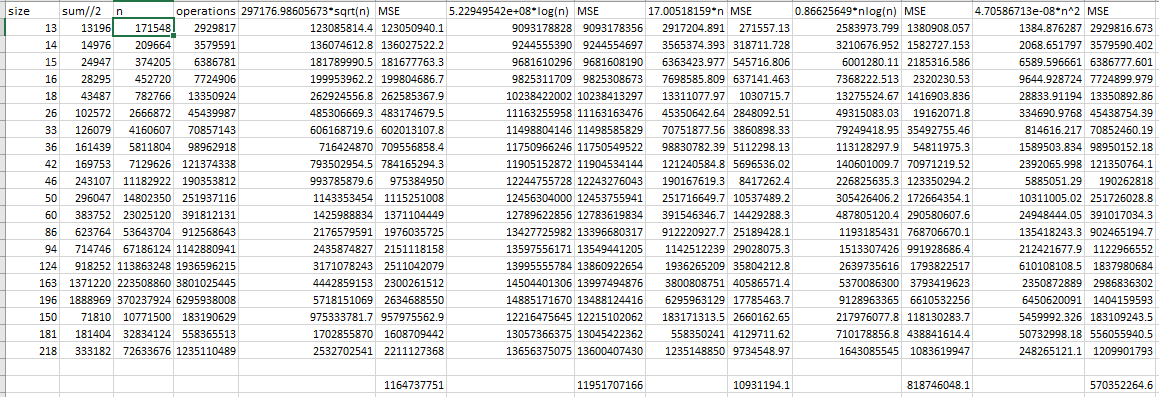
\includegraphics[width=\textwidth,height=\textheight,keepaspectratio]{bang.png}

trong đó: sum: tổng các phần tử trong list

          size: số phần tử trong list
          
          n: sum*size
          
MSE: 
\begin{itemize}
    \item $\sqrt{sum*size} = 1164737751$
    \item $\log{(sum*size)} = 11951707166$
    \item sum*size = 10931194.11
    \item sum*size * $\log{(sum*size)} = 818746048.1$
    \item \((sum*size)^2\) = 570352264.6
\end{itemize}

Có thể thấy MSE của sum*size là bé nhất, như vậy độ phức tạp của thuật toán theo thực nghiệm là O(sum*size), bằng với độ phức tạp phân tích lý thuyết.

\subsection{Thuật toán tối ưu hóa không gian}
Thay vì tạo một mảng 2 chiều có kích thước bằng (size+1)*(sum/2 +1)
Tạo một mảng với số phần tử bằng sum/2. + 1 Phần tử thứ j sẽ là True có tập hợp con có tổng bằng j, ngược lại là False.
Do đó độ phức tạp không gian là O(sum).\\

\textbf{Điều kiện:} size*sum < $10^{10}$\\

\textbf{Mã giả:} 
Partition(arr, sum):
\begin{enumerate}
    \item n = len(arr)
    \item sum = 0
    \item For i=0 to n : sum+=arr[i]
    \item If sum div 2 != 0 : return False 
    \item Initalize Part = [False] * ((sum//2)+1)
    \item \setlength{\itemindent}{40pt} For i to n:
   \item \setlength{\itemindent}{80pt}  For j =  Sum//2 to arr[i] -1 :
      
      \item  \setlength{\itemindent}{1500pt}Part[j] = True If Part[j - arr[i]] == True | j == arr[i]
       \item \noindent Return Part[Sum//2]
\end{enumerate}
\textbf{Phân tích độ phức tạp bằng phân tích lý thuyết}
\begin{itemize}
    \item Tại dòng 1,2: phép gán => độ phức tạp 2
    \item Dòng 3: vòng lặp từ 0 đến n và phép gán trong mỗi vòng lặp => độ phức tạp n
    \item Dòng 4: phép chia và so sánh => độ phức tạp là 2
    \item Dòng 5: khởi tạo mảng Part với kích thước sum//2 + 1 và gán cho các phần tử của Part => độ phức tạp là sum
    \item Dòng 6,7,8 khởi tạo 2 vòng lặp từ 0 đến n và từ sum//2 đến arr[i] - 1 => độ phức tạp là sum*n
\end{itemize}
Độ phức tạp của thuật toán: sum*n + sum + n + 2 + 2

Áp dụng quy tắc lấy Max: độ phức tạp: O(sum*n)\\
\textbf{Thực nghiệm:}\\
\noindent \includegraphics[width=\textwidth,height=\textheight,keepaspectratio]{opti.png}

trong đó: sum: tổng các phần tử trong list

          size: số phần tử trong list
          
          n: sum*size
          
MSE: 
\begin{itemize}
    \item $\sqrt{sum*size} = 60450445484$
    \item $\log{(sum*size)} = 5.79534E+11$
    \item sum*size = 2211888482
    \item sum*size * $\log{(sum*size)} = 10485616375$
    \item \((sum*size)^2\) = 4.3106E+11
\end{itemize}

Có thể thấy sum*size có MSE bé nhất phù hợp với độ phức tạp lý thuyết của thuật toán.
\subsection{Trace back tìm subset}
Bài toán nâng cấp từ number partition: Áp dụng bài toán trên để tìm ra 2 subset có tổng bằng nhau. Thực hiện traceback từ ma trận đã tạo của number partition.
\begin{itemize}
    \item Input: ma trận partition part, tổng các phần tử trong list sum, list arr
    \item Output: 2 subset có tổng bằng sum/2.
\end{itemize}
\textbf{Mã giả:}\\
Traceback(part, sum, arr):
\begin{enumerate}
    \item tong = 0 
    \item index = len(part) - 1
    \item path = []
    \item \setlength{\itemindent}{40pt} while tong!= sum:
    \item i = part[index].index(True) - 1
    \item tong += arr[i]
    \item path.append(i)
    \item index -= arr[i]
    \item \noindent Initalize S1 = [], S2 = []
    \item \noindent for i = 0 to len(arr):
    \item S1.append(arr[i]) if i in path
    \item else: S2.append(arr[i])
    \item \noindent return S1, S2
\end{enumerate}
\subsection{Tham khảo}
\begin{enumerate}
    \item https://www.geeksforgeeks.org/partition-problem-dp-18
    \item https://en.wikipedia.org/wiki/Partition\_problem
\end{enumerate}

\end{document}